\documentclass[12pt,final]{report}


% change values of these variables
\newcommand{\thesistitle}{Thesis Title}
\newcommand{\authorname}{Your name}
\newcommand{\authorroll}{1603***}
\newcommand{\thesissupervisor}{Supervisor Name}
\newcommand{\thesissupervisordesignation}{Supervisor Designation}
\newcommand{\external}{External Name}
\newcommand{\externaldesig}{External Designation}
\newcommand{\tarikh}{October 16, 2022}

% donot change
\usepackage{packages}
\newcommand{\dept}{Department of Computer Science \& Engineering}
\newcommand{\ruet}{Rajshahi University of Engineering \& Technology}


\begin{document}

% skips page number on title page
\pagenumbering{gobble}
\begin{center}
    \textit{Heaven's Light is Our Guide}
    \vspace{1cm}
    
    % 
\includegraphics[height=4cm]{imgs/ruetlogo.pdf}
    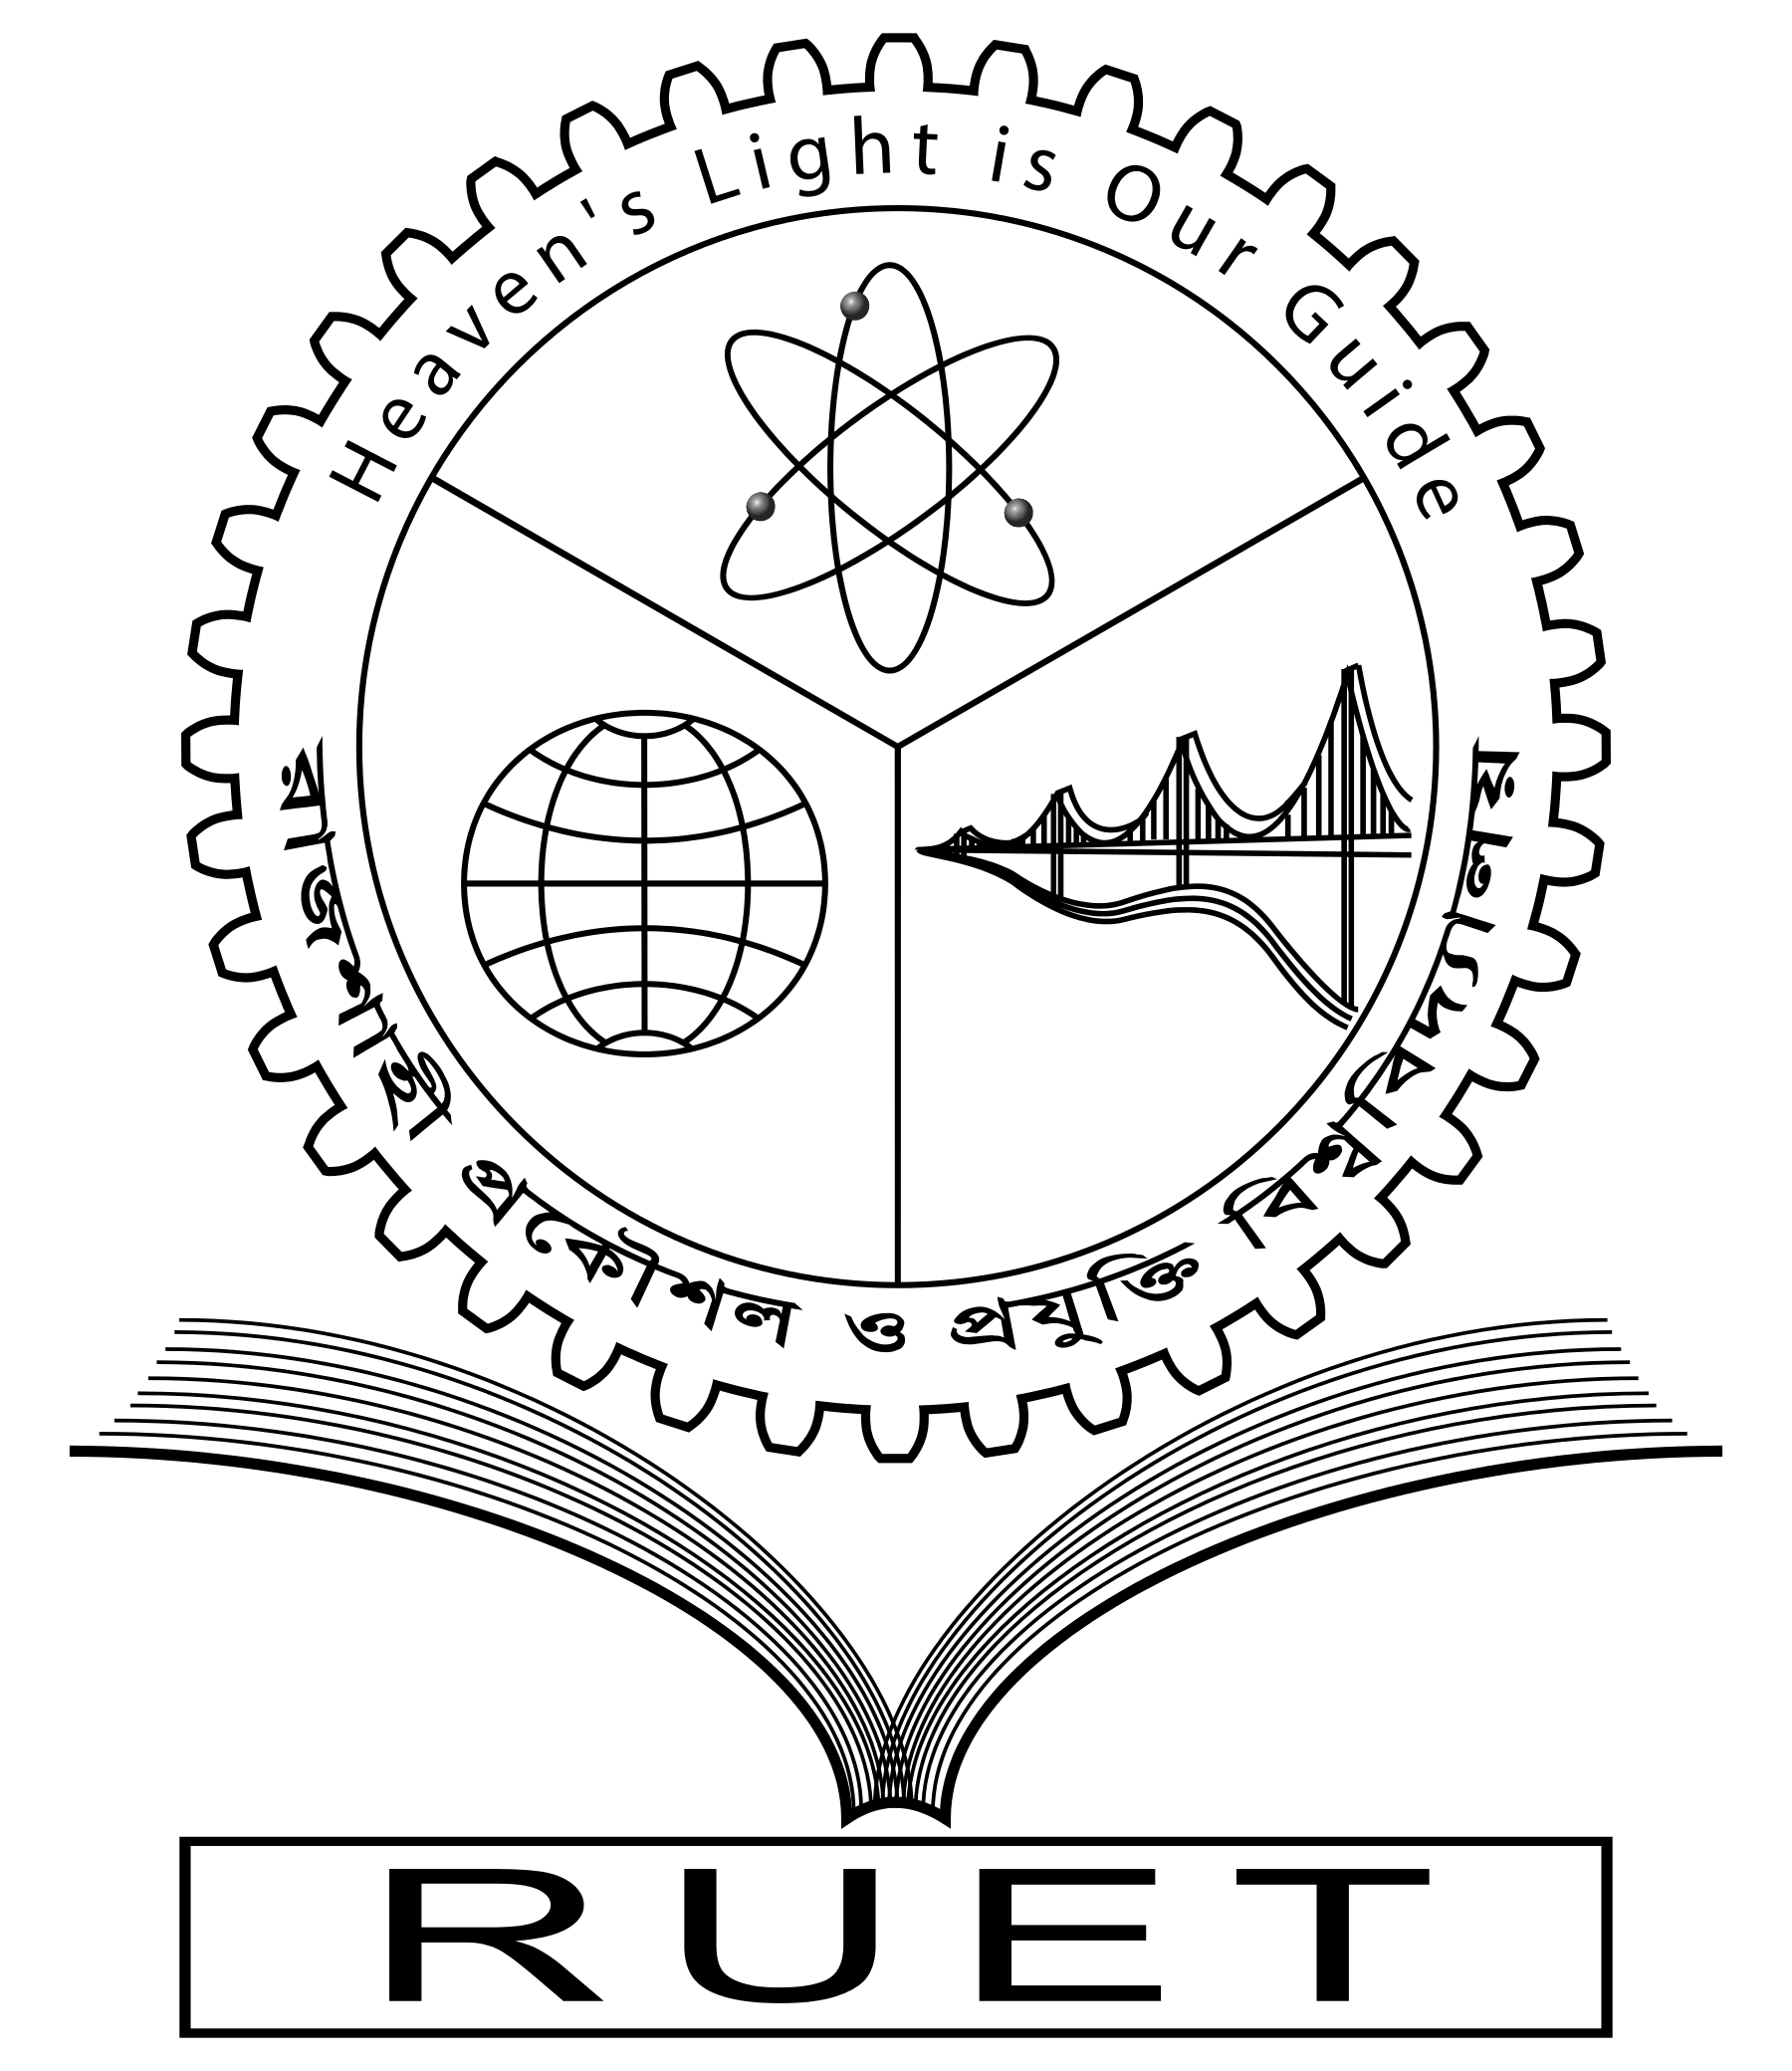
\includegraphics[height=4cm]{imgs/RUET_logo_bw.png}
    \vspace{1cm}
    
    \textbf{{\fontsize{14pt}{0.5cm}\selectfont \dept}}
    \vspace{1cm}
    
    \textbf{{\fontsize{14pt}{0.5cm}\selectfont \ruet, Bangladesh}}
    \vspace{1cm}

    \textbf{{\fontsize{16pt}{0.5cm}\selectfont \thesistitle}}
    \vspace{1cm}

    {\fontsize{14pt}{0.5cm}\selectfont
        \textbf{Author}\\
        \authorname\\
        Roll No. \authorroll\\
        \dept\\
        \ruet\\
        \vspace{1cm}

        \textbf{Supervised by}\\
        \thesissupervisor\\
        \thesissupervisordesignation\\
        \dept\\
        \ruet\\
        \vspace{1cm}
    }

\end{center}
\clearpage
\pagenumbering{roman}
\setcounter{page}{2}
\addcontentsline{toc}{chapter}{ACKNOWLEDGEMENT}
\begin{center}
        \textbf{{\fontsize{16pt}{0.5cm}\selectfont ACKNOWLEDGEMENT}}
        \vspace{1cm}
\end{center}

\noindent% edit area start
\lipsum[1-1]
% edit area end

\vfill


{\fontsize{14pt}{17}\selectfont
        \begin{tabular}{>{\raggedright}p{0.48\linewidth}>{\raggedleft}p{0.48\linewidth}}
                \tarikh         & \authorname
                \tabularnewline 
                RUET, Rajshahi  &
                \tabularnewline            
        \end{tabular}
}

\clearpage
\addcontentsline{toc}{chapter}{CERTIFICATE}

\begin{center}
    \textit{Heaven's Light is Our Guide}
    \vspace{8mm}

    
\includegraphics[height=4cm]{imgs/ruetlogo.pdf}
    \vspace{8mm}
    
    \textbf{{\fontsize{14pt}{0.5cm}\selectfont \dept}}
    \vspace{8mm}
    
    \textbf{{\fontsize{14pt}{0.5cm}\selectfont \ruet}}
    \vspace{8mm}

    \textbf{{\fontsize{16pt}{0.5cm}\selectfont \textit{CERTIFICATE}}}
    \vspace{8mm}
\end{center}

\noindent\textit{% edit area start
This is to certify that the thesis entitled \textbf{“\thesistitle”} has been carried out by \textbf{\authorname, Roll: \authorroll}\ in partial fulfillment of the requirement for the award of the degree of Bachelor of Science in the \dept\ at \ruet, Rajshahi, Bangladesh, is a record of the candidate's own work carried out by him under my supervision. This thesis has not been submitted for the award of any other degree.
% edit area end
}

% \vspace{1cm}
\vfill

\begin{minipage}{0.45\linewidth}
    Supervisor\\
    \hfill\\
    \hrule
    \hfill\\
    \textbf{\thesissupervisor}\\
    \thesissupervisordesignation\\
    \dept\\
    \ruet\\
    Rajshahi-6204
\end{minipage}
\hfill
\begin{minipage}{0.45\linewidth}
    External Examiner\\
    \hfill\\
    \hrule
    \hfill\\
    \textbf{\external}\\
    \externaldesig\\
    \dept\\
    \ruet\\
    Rajshahi-6204
\end{minipage}
\addcontentsline{toc}{chapter}{ABSTRACT}
\begin{center}
        \textbf{{\fontsize{16pt}{18}\selectfont ABSTRACT}}
        \vspace{1cm}
\end{center}

\noindent%edita area start
\lipsum[1]
%edit area end

\clearpage


\tableofcontents
\newpage
% comment-out the marked lines, if you want your "list of tables" and "list of figures" in different pages
\listoftables
\begingroup % mark
    \let\cleardoublepage\relax % mark
    \let\clearpage\relax % mark
    \listoffigures
\endgroup % mark
\clearpage

\pagenumbering{arabic}
\chapter{Introduction}
\noindent Rajshahi University of Engineering \& Technology \cite{ruetwebsite}, formerly known as BIT Rajshahi, is the second oldest engineering university in Bangladesh. It was founded in 1964 as a faculty of Engineering under the University of Rajshahi.

\section{Something}
\noindent Lorem ipsum \cite{awesome2016} dolor sit amet, consectetur adipiscing elit, sed do eiusmod tempor incididunt ut labore et dolore magna aliqua. Ut enim ad minim veniam, quis nostrud exercitation ullamco laboris nisi ut aliquip ex ea commodo consequat. Duis aute irure dolor in reprehenderit in voluptate velit esse cillum dolore eu fugiat nulla pariatur. Excepteur sint occaecat cupidatat non proident, sunt in culpa qui officia deserunt mollit anim id est laborum.

\subsection{Applications of Something}

\begin{enumerate}
        \item Application One
        \item Application Two
        \item Application Three
\end{enumerate}

\section{Organization}
Excepteur sint occaecat cupidatat non proident, sunt in culpa qui officia deserunt mollit anim id est laborum.

\begin{description}
        \item[Chapter 1] \hfill \\
        Lorem ipsum dolor sit amet
        \item[Chapter 2] \hfill \\
        Consectetur adipiscing elit
        \item[Chapter 3] \hfill \\
        Sed do eiusmod tempor incididunt ut labore et dolore magna aliqua
        \item[Chapter 4] \hfill \\
        Ut enim ad minim veniam
        \item[Chapter 5] \hfill \\
        Quis nostrud exercitation ullamco laboris nisi ut aliquip ex ea commodo consequat
\end{description}

\section*{Conclusion}
\addcontentsline{toc}{section}{Conclusion}
\lipsum[1]
\chapter{Background}

\section{Introduction}
\noindent Lorem ipsum dolor sit amet, consectetur adipiscing elit, sed do eiusmod tempor incididunt ut labore et dolore magna aliqua. Ut enim ad minim veniam, quis nostrud exercitation ullamco laboris nisi ut aliquip ex ea commodo consequat. Duis aute irure dolor in reprehenderit in voluptate velit esse cillum dolore eu fugiat nulla pariatur. Excepteur sint occaecat cupidatat non proident, sunt in culpa qui officia deserunt mollit anim id est laborum.

\section{Some Section}
\noindent Lorem ipsum dolor sit amet, consectetur adipiscing elit, sed do eiusmod tempor incididunt ut labore et dolore magna aliqua. Ut enim ad minim veniam, quis nostrud exercitation ullamco laboris nisi ut aliquip ex ea commodo consequat. Duis aute irure dolor in reprehenderit in voluptate velit esse cillum dolore eu fugiat nulla pariatur. Excepteur sint occaecat cupidatat non proident, sunt in culpa qui officia deserunt mollit anim id est laborum.

\begin{figure}[H]
        \centering
        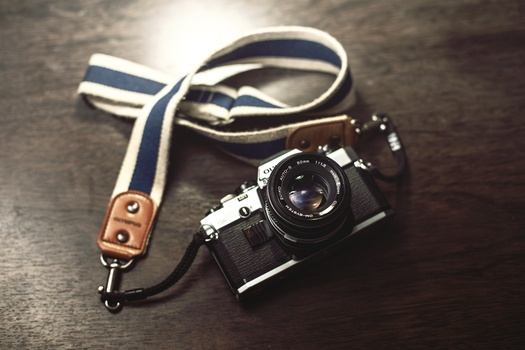
\includegraphics[width=3in]{imgs/camera.jpg}
        \caption[A Camera]
        {A Camera}
\end{figure}

\noindent Lorem ipsum dolor sit amet, consectetur adipiscing elit, sed do eiusmod tempor incididunt ut labore et dolore magna aliqua. Ut enim ad minim veniam, quis nostrud exercitation ullamco laboris nisi ut aliquip ex ea commodo consequat. Duis aute irure dolor in reprehenderit in voluptate velit esse cillum dolore eu fugiat nulla pariatur. Excepteur sint occaecat cupidatat non proident, sunt in culpa qui officia deserunt mollit anim id est laborum.

\begin{figure}[H]
        \centering
        \begin{subfigure}[b]{0.4\textwidth}
                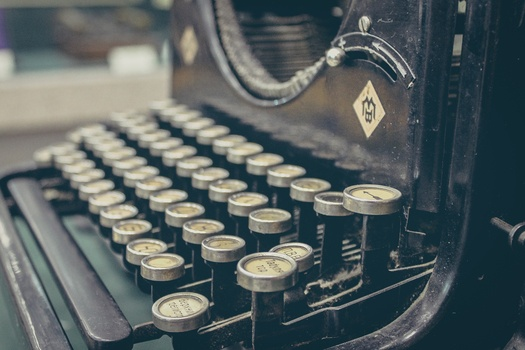
\includegraphics[width=\textwidth]{imgs/typewriter.jpg}
                \caption{A Typewriter}
                \label{fig:typewriter}
        \end{subfigure}
        \begin{subfigure}[b]{0.4\textwidth}
                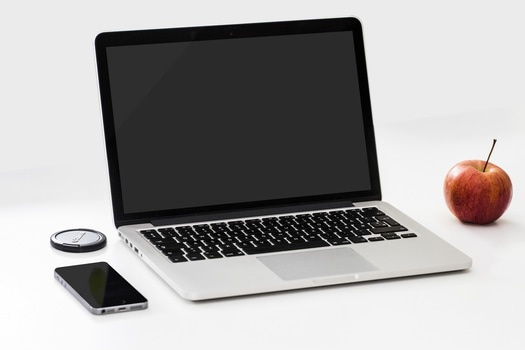
\includegraphics[width=\textwidth]{imgs/macbookpro.jpg}
                \caption{A Macbookpro}
                \label{fig:macbookpro}
        \end{subfigure}
        \caption{Typewriter and Macbookpro}\label{fig:typewriter_macbookpro}
\end{figure}

\chapter{Implementation}

\noindent Lorem ipsum dolor sit amet, consectetur adipiscing elit, sed do eiusmod tempor incididunt ut labore et dolore magna aliqua. Ut enim ad minim veniam, quis nostrud exercitation ullamco laboris nisi ut aliquip ex ea commodo consequat. Duis aute irure dolor in reprehenderit in voluptate velit esse cillum dolore eu fugiat nulla pariatur. Excepteur sint occaecat cupidatat non proident, sunt in culpa qui officia deserunt mollit anim id est laborum.

\section{Some Section}
\noindent Lorem ipsum dolor sit amet, consectetur adipiscing elit, sed do eiusmod tempor incididunt ut labore et dolore magna aliqua. Ut enim ad minim veniam, quis nostrud exercitation ullamco laboris nisi ut aliquip ex ea commodo consequat. Duis aute irure dolor in reprehenderit in voluptate velit esse cillum dolore eu fugiat nulla pariatur. Excepteur sint occaecat cupidatat non proident, sunt in culpa qui officia deserunt mollit anim id est laborum.

\subsection{Some Subsection}
\noindent Lorem ipsum dolor sit amet, consectetur adipiscing elit, sed do eiusmod tempor incididunt ut labore et dolore magna aliqua. Ut enim ad minim veniam, quis nostrud exercitation ullamco laboris nisi ut aliquip ex ea commodo consequat.

\chapter{Result and Performence Analysis}

\section{Result}

\noindent Lorem ipsum dolor sit amet, consectetur adipiscing elit, sed do eiusmod tempor incididunt ut labore et dolore magna aliqua. Ut enim ad minim veniam, quis nostrud exercitation ullamco laboris nisi ut aliquip ex ea commodo consequat. Duis aute irure dolor in reprehenderit in voluptate velit esse cillum dolore eu fugiat nulla pariatur. Excepteur sint occaecat cupidatat non proident, sunt in culpa qui officia deserunt mollit anim id est laborum.\newline

\begin{table}[H]
        \caption{List of the largest information technology companies}
        \begin{center}
                \begin{tabular}{|l|l|c|}\hline
                        Rank & Company             & Revenue     \\ \hline
                        1    & Apple Inc.          & \$233.715 B \\ \hline
                        2    & Samsung Electronics & \$189.500 B \\ \hline
                        3    & Foxconn             & \$132.070 B \\ \hline
                        4    & HP                  & \$111.450 B \\ \hline
                        5    & Microsoft           & \$093.580 B \\ \hline
                        6    & IBM                 & \$092.790 B \\ \hline
                \end{tabular}
        \end{center}
        \label{tab:result}
\end{table}

\section{Performence Analysis}
\noindent Lorem ipsum dolor sit amet, consectetur adipiscing elit, sed do eiusmod tempor incididunt ut labore et dolore magna aliqua. Ut enim ad minim veniam, quis nostrud exercitation ullamco laboris nisi ut aliquip ex ea commodo consequat. Duis aute irure dolor in reprehenderit in voluptate velit esse cillum dolore eu fugiat nulla pariatur. Excepteur sint occaecat cupidatat non proident, sunt in culpa qui officia deserunt mollit anim id est laborum.

\chapter{Conclusion and Future Works}

\section{Conclusion}

\noindent Lorem ipsum dolor sit amet, consectetur adipiscing elit, sed do eiusmod tempor incididunt ut labore et dolore magna aliqua. Ut enim ad minim veniam, quis nostrud exercitation ullamco laboris nisi ut aliquip ex ea commodo consequat. Duis aute irure dolor in reprehenderit in voluptate velit esse cillum dolore eu fugiat nulla pariatur. Excepteur sint occaecat cupidatat non proident, sunt in culpa qui officia deserunt mollit anim id est laborum.

\section{Future Works}

\noindent Lorem ipsum dolor sit amet, consectetur adipiscing elit, sed do eiusmod tempor incididunt ut labore et dolore magna aliqua. Ut enim ad minim veniam, quis nostrud exercitation ullamco laboris nisi ut aliquip ex ea commodo consequat. Duis aute irure dolor in reprehenderit in voluptate velit esse cillum dolore eu fugiat nulla pariatur. Excepteur sint occaecat cupidatat non proident, sunt in culpa qui officia deserunt mollit anim id est laborum.

\begin{appendices}

\chapter{Code Snippets}
\section{HelloWorld.c}
\begin{minted}{c++}
#include <iostream>
using namesapce std;
int main(void){
    cout << "Hello World" << endl;
    return 0;
}
\end{minted}

\end{appendices}


% \nocite{*}
\printbibliography[heading=bibintoc,title={REFERENCES}]

\end{document}
